\documentclass[14pt]{extreport}
\usepackage{gost}
\usepackage{hyperref}
\usepackage{makecell}
\usepackage{ragged2e}
\usepackage{graphicx}%Вставка картинок правильная
\usepackage{float}%"Плавающие" картинки
\usepackage{wrapfig}%Обтекание фигур (таблиц, картинок и прочего)
	
\usepackage{lscape}
\justifying
\makeatletter
\@addtoreset{figure}{part}% Reset figure numbering at every part
\makeatother
\renewcommand{\thefigure}{\arabic{figure}}% Figure number is part.figure
\renewcommand{\thetable}{\arabic{table}}



%Тут можно вставить дополнительные пакеты

\begin{document}
\pagestyle{empty} %  выключаем нумерацию

\includepdf[pages=-,pagecommand={}]{titlePage.pdf}


\pagestyle{plain} % включаем нумерацию
\tableofcontents
\intro\label{intro} 

В данной лабораторной работе была реализована система обработки данных <<Программа для контроля собственных денежных средств>>, а так же проанализирована предметная область и требования к работе.

\chapter{Анализ}
\section{Анализ предметной области}

На рынке представлено множество программного обеспечения со схожим функционалом. Их можно разделить на несколько типов: мобильные приложения банков, приложения для ручного ввода трат, приложения которые синхронизируются с банковскими приложениями. Все представленное на рынке программное обеспечение имеет следующий общий функционал: ручное/автоматическое добавление транзакций, удаление, отображение транзакций по дате, отображение транзакций по категориям, сортировка по другим параметрам. Учитывая рост спроса на потребительские товары и услуги по всему миру, область перспективной, а разработку данной программной модели - актуальной.

\section{Анализ требований}

Проанализировав предметную область, а так же задание полученное на практике по дисциплине <<Программирование>>, были выдвинуты следующие технические требования к программной модели: 
\begin{enumerate}
    \item Разработать алгоритм работы системы
    \item Спроектировать базу данных SQLite3
    \item Разработать веб-сервер для статических файлов с помощью языка программирования Python и библиотеки Flask
    \item Разработать веб-сервер для обработки POST и GET запросов.
    \item Разработать веб-интерфейс для программной модели.
\end{enumerate}

\chapter{Ход работы}
\section{Разработка алгоритма работы системы}
Для разрабатываемой модели программной системы был разработан и представлен в виде блок-схемы следующий алгоритм. (Рисунок \ref{fig:d0}).
\begin{figure}[h]   
    \centering
    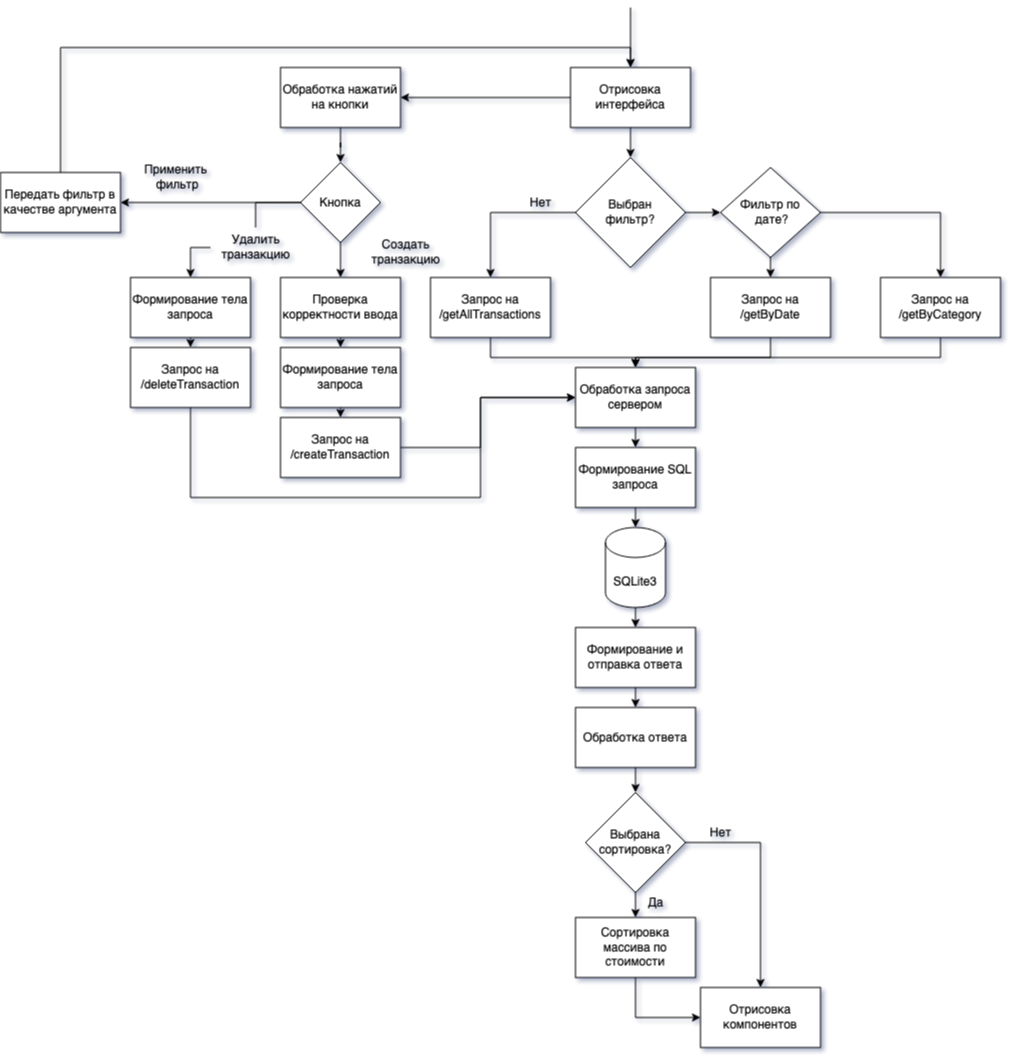
\includegraphics[width=1\linewidth]{block.png}
    \caption{ Блок-схема алгоритма }
    \label{fig:d0}
\end{figure}
\section{Проектирование базы данных SQLite3}

Для разработки модели программной системы было решено использовать систему управления базами данных SQLite3. Данная СУБД имеет такие преимущества, как: высокая скорость, кроссплатформенность, надежность, а так же не нуждается в конфигурации. 

Для хранения транзакций была спроектирована следуящая модель базы данных. Модель включает в себя одну таблицу <<transactions>>, записи в которой имеют такие свойства, как: 
\begin{enumerate}
    \item tr-id - id транзакции, так же является primary key для таблицы (integer)
    \item name - название транзакции (string)
    \item cost - стоимость транзакции (integer)
    \item date - дата транзакции. Для хранения дат было приято решение хранить их в формате unix-time. (integer)
    \item category - категория транзакции (string)
\end{enumerate}

Ниже демонстрируется схема базы данных (Рисунок \ref{fig:d1}). 

\begin{figure}[h]   
    \centering
    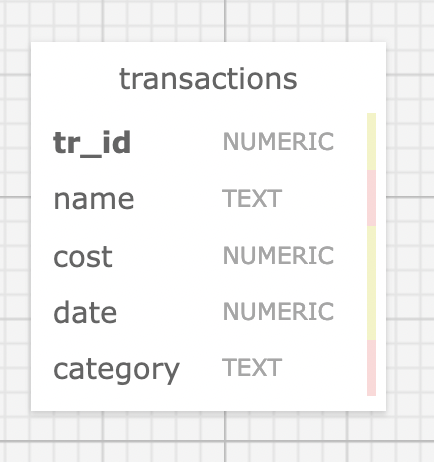
\includegraphics[width=0.5\linewidth]{db.png}
    \caption{ Схема базы данных }
    \label{fig:d1}
\end{figure}

\section{Разраотка сервера для статических файлов}

Для реализации модели программной системы используется высокоуровневый язык программирования Python. Для ускорения процесса разработки было принято использовать фреймворк для создания веб-приложений Flask.

Для корректной работы программной модели был разработан сервер статических файлов с помощью библиотеки Flask. Сервер работает на порту 5000, рабочей директорией для него является <<./www/>>. Сервер устанавливает MIME-типы для файлов формата html, css, js. Ниже представлен фрагмет кода на языке программирования Python. (Рисунок \ref{fig:d2}). 

\begin{figure}[h]   
    \centering
    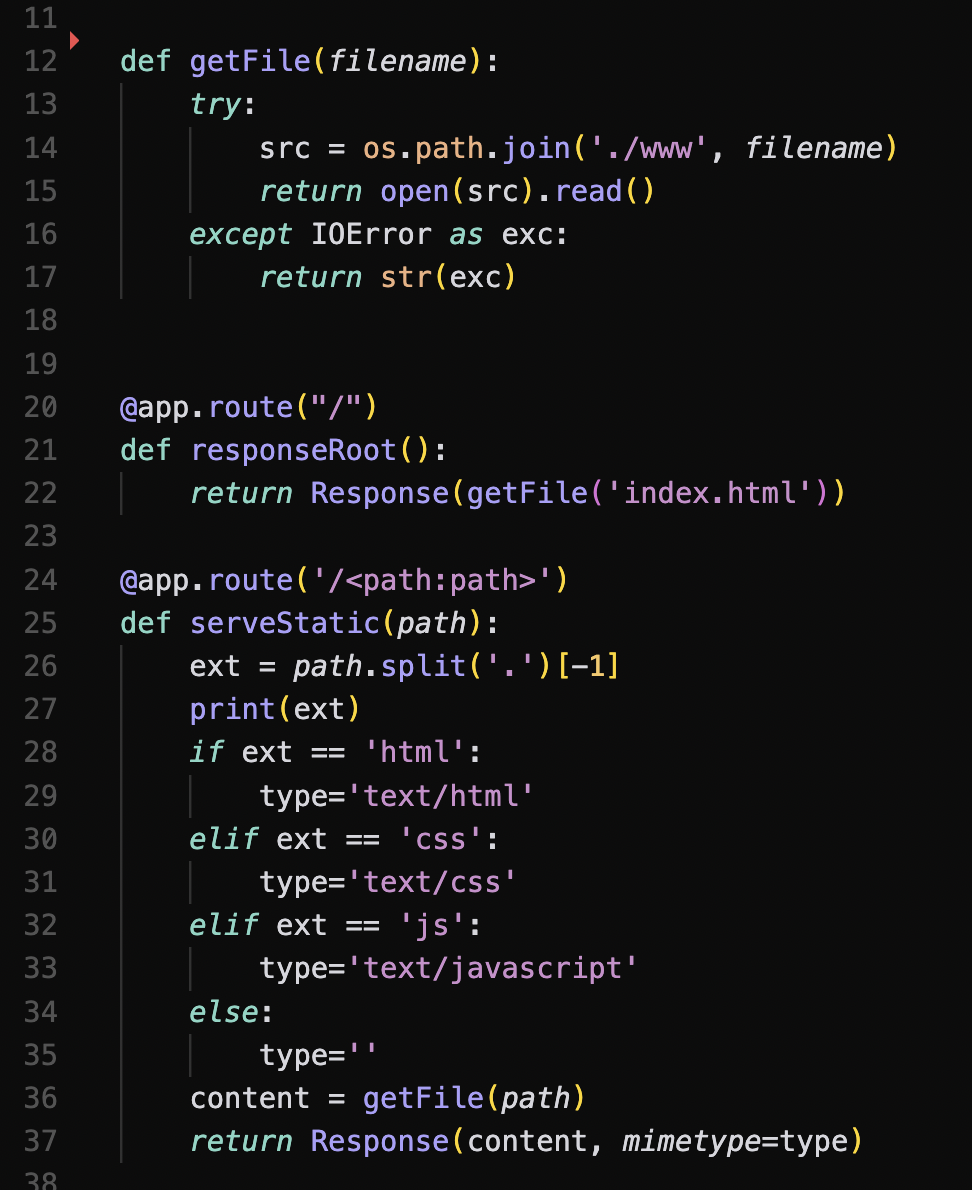
\includegraphics[width=0.5\linewidth]{static1.png}
    \caption{ Фрагмент кода сервера статических файлов }
    \label{fig:d2}
\end{figure}

В качестве интерфейса для программной модели было принято решение использовать веб интерфейс. Веб интерфейс расположен в директории <<./www/>> и имеет главную страницу на языке разметки гипертекста, каскадную таблицу стилей, а так же логика работы описана на языке программирования высокого уровня JavaScript. В результате веб-интерфейс будет доступен по адресу http://localhost:5000.

\section{Разработка сервера для обработки POST и GET запросов }

Аналогично, для реализации веб-сервера для обработки POST и GET запросов был использован язык программирования высокого уровня Python, а так же библиотека для разработки веб-приложений Flask.

Для реализации обработки GET запросов был написан следующий код.  (Рисунок \ref{fig:d3}). 

\begin{figure}[h]   
    \centering
    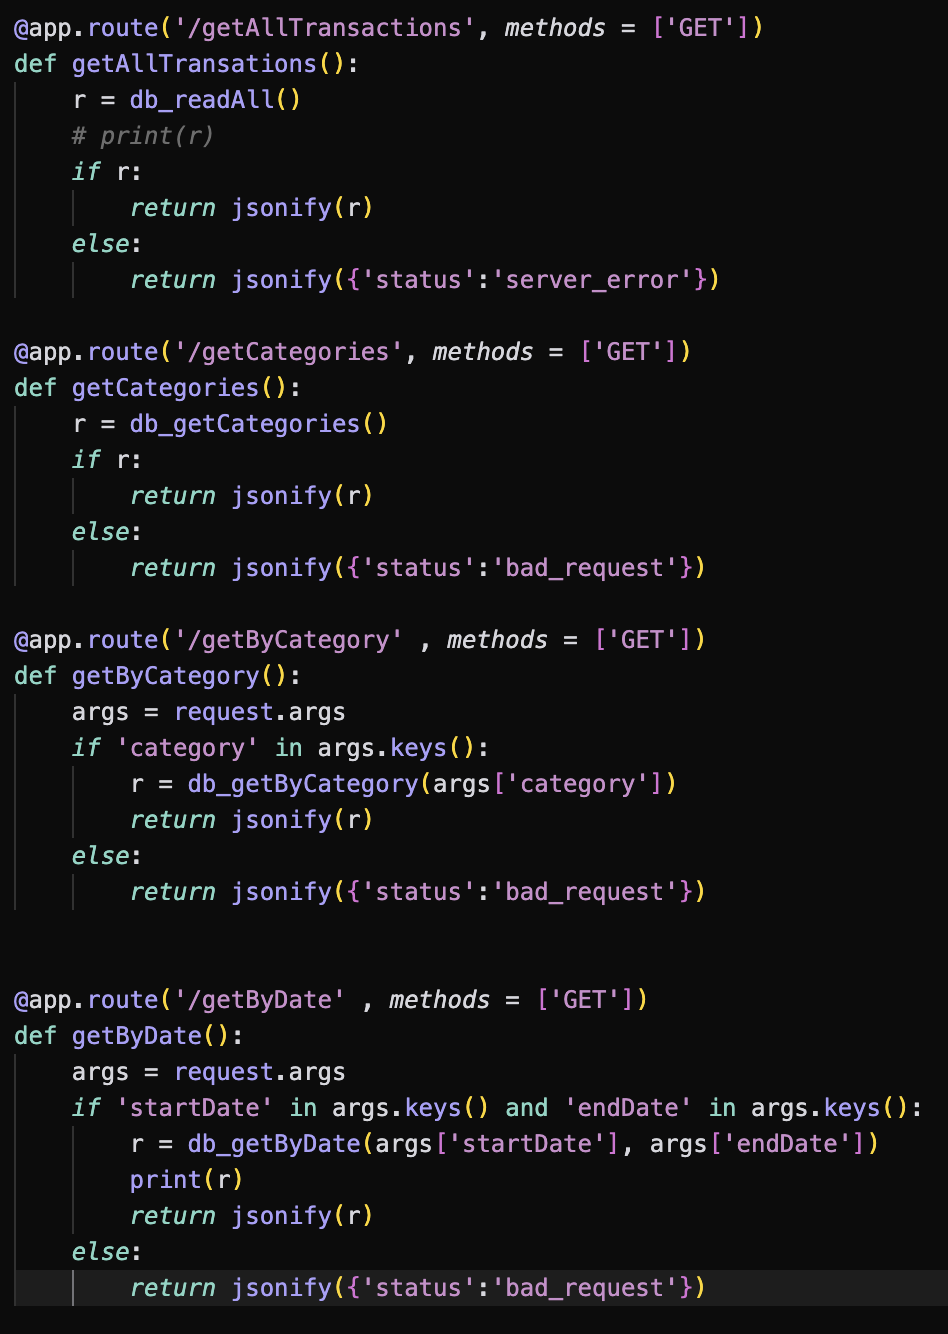
\includegraphics[width=0.5\linewidth]{get.png}
    \caption{ Фрагмент кода для обработки GET запросов }
    \label{fig:d3}
\end{figure}

В представленном фрагменте кода обрабатываются GET запросы по адресам <</getAllTransactions>> (возвращает все транзакции), <</getCategories>> (возвращает категории), <</getByCategory>> (возвращает транзакции по определенной категории) и <</getByDate>> (возвращает транзакции за заданный временной период). Получая запрос, осуществляется запрос к базе данных SQLite3. Возможность обращения к базе данных реализована в отдельном файле db.py.  (Рисунок \ref{fig:d5}). Получая ответ от базы данных, обрабатываются ошибки и возвращается ответ на запрос в формате JSON.
\\

Так же, для реализации обработки POST запросов, был реализован следующий код. (Рисунок \ref{fig:d4})

\begin{figure}[h]   
    \centering
    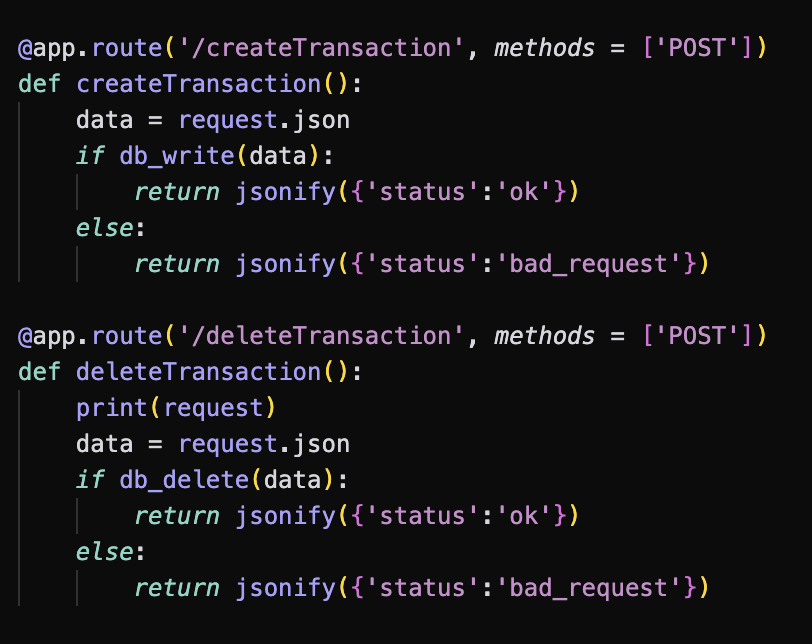
\includegraphics[width=0.4\linewidth]{post.png}
    \caption{ Фрагмент кода для обработки POST запросов }
    \label{fig:d4}
\end{figure}

В представленном фрагменте кода представлена реализация обработки POST запросов. Запросы обрабатываются по адресам <</createTransaction>> и <</deleteTransaction>>. В теле запроса передается информация о транзакции. Корректность тела запроса проверяется, далее идет запрос к базе данных SQLite3. В результате возвращается ответ в формате JSON.
\\ 

Для реалзизации возможности работы с базой данных SQLite3 была написана следующая функция для работы с базой данных (Рисунок \ref{fig:d5}). Для реализации функции была использована библиотека sqlite3. 

\begin{figure}[h]   
    \centering
    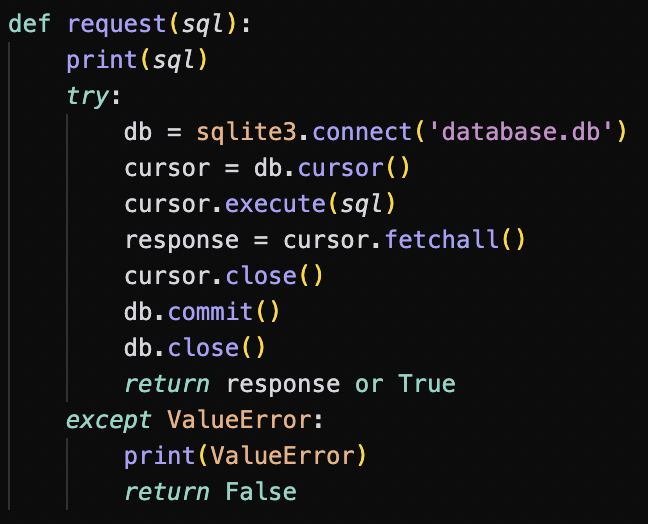
\includegraphics[width=0.4\linewidth]{db2.png}
    \caption{ Фрагмент кода для работы с базой данных }
    \label{fig:d5}
\end{figure}

В приведенном фрагменте функция получает на вход строку - SQL запрос, и выполняет его для базы данных databse.db. В случае ошибки функция возвращает False, в случае успешного выполнения запроса функция возвращает True или результат выполнения запроса (если он присутствует)

Для обработки каждого GET и POST запроса был написан соответствующий SQL запрос, соответствующие функции реализованы в файле db.py.

\section{Разработка веб-интерфейса для программной модели}

Для реализации взаимодействия пользователя с программой был выбран веб-интерфейс. Веб-интерфейс реализован с помощью языка разметки гипертекста HTML, каскадных таблиц стилей CSS, а так же языка программирования высокого уровня JavaScript. Веб-интерфейс отображается при GET запросе к серверу статических файлов по адресу http://localhost:5000. Код на языке JavaScript осуществляет работу логики приложения и осуществляет POST и GET запросы к веб-серверу написанному с помощью языка Python.

В представленном ниже фрагменте кода (Рисунок \ref{fig:d6}) демонстрируется функция отправка HTTP запроса написанная на языке JavaScript. 

\begin{figure}[h]   
    \centering
    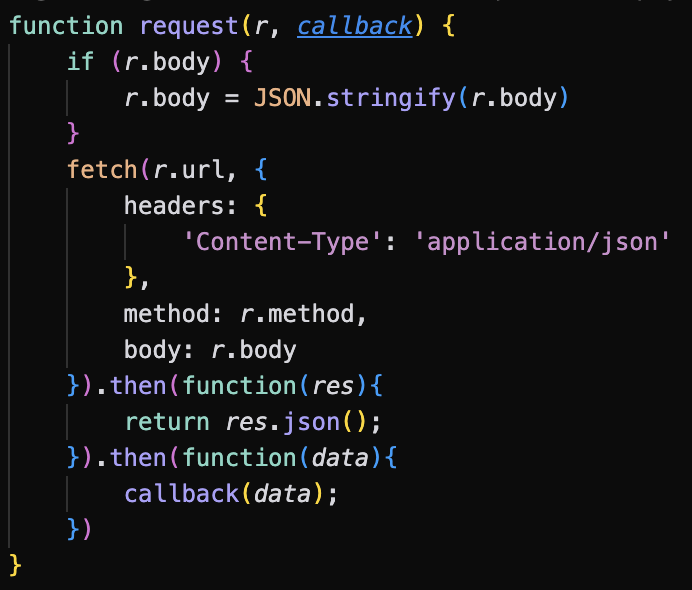
\includegraphics[width=0.4\linewidth]{js.png}
    \caption{ Фрагмент кода для отправки HTTP запроса }
    \label{fig:d6}
\end{figure}

Функция принимает в качестве аргумента объект r с параметрами, а так же функцию callback.

\newpage 

Итоговый внешний вид программной модели выглядит следующим образом: (Рисунок \ref{fig:d7})
\begin{figure}[h]   
    \centering
    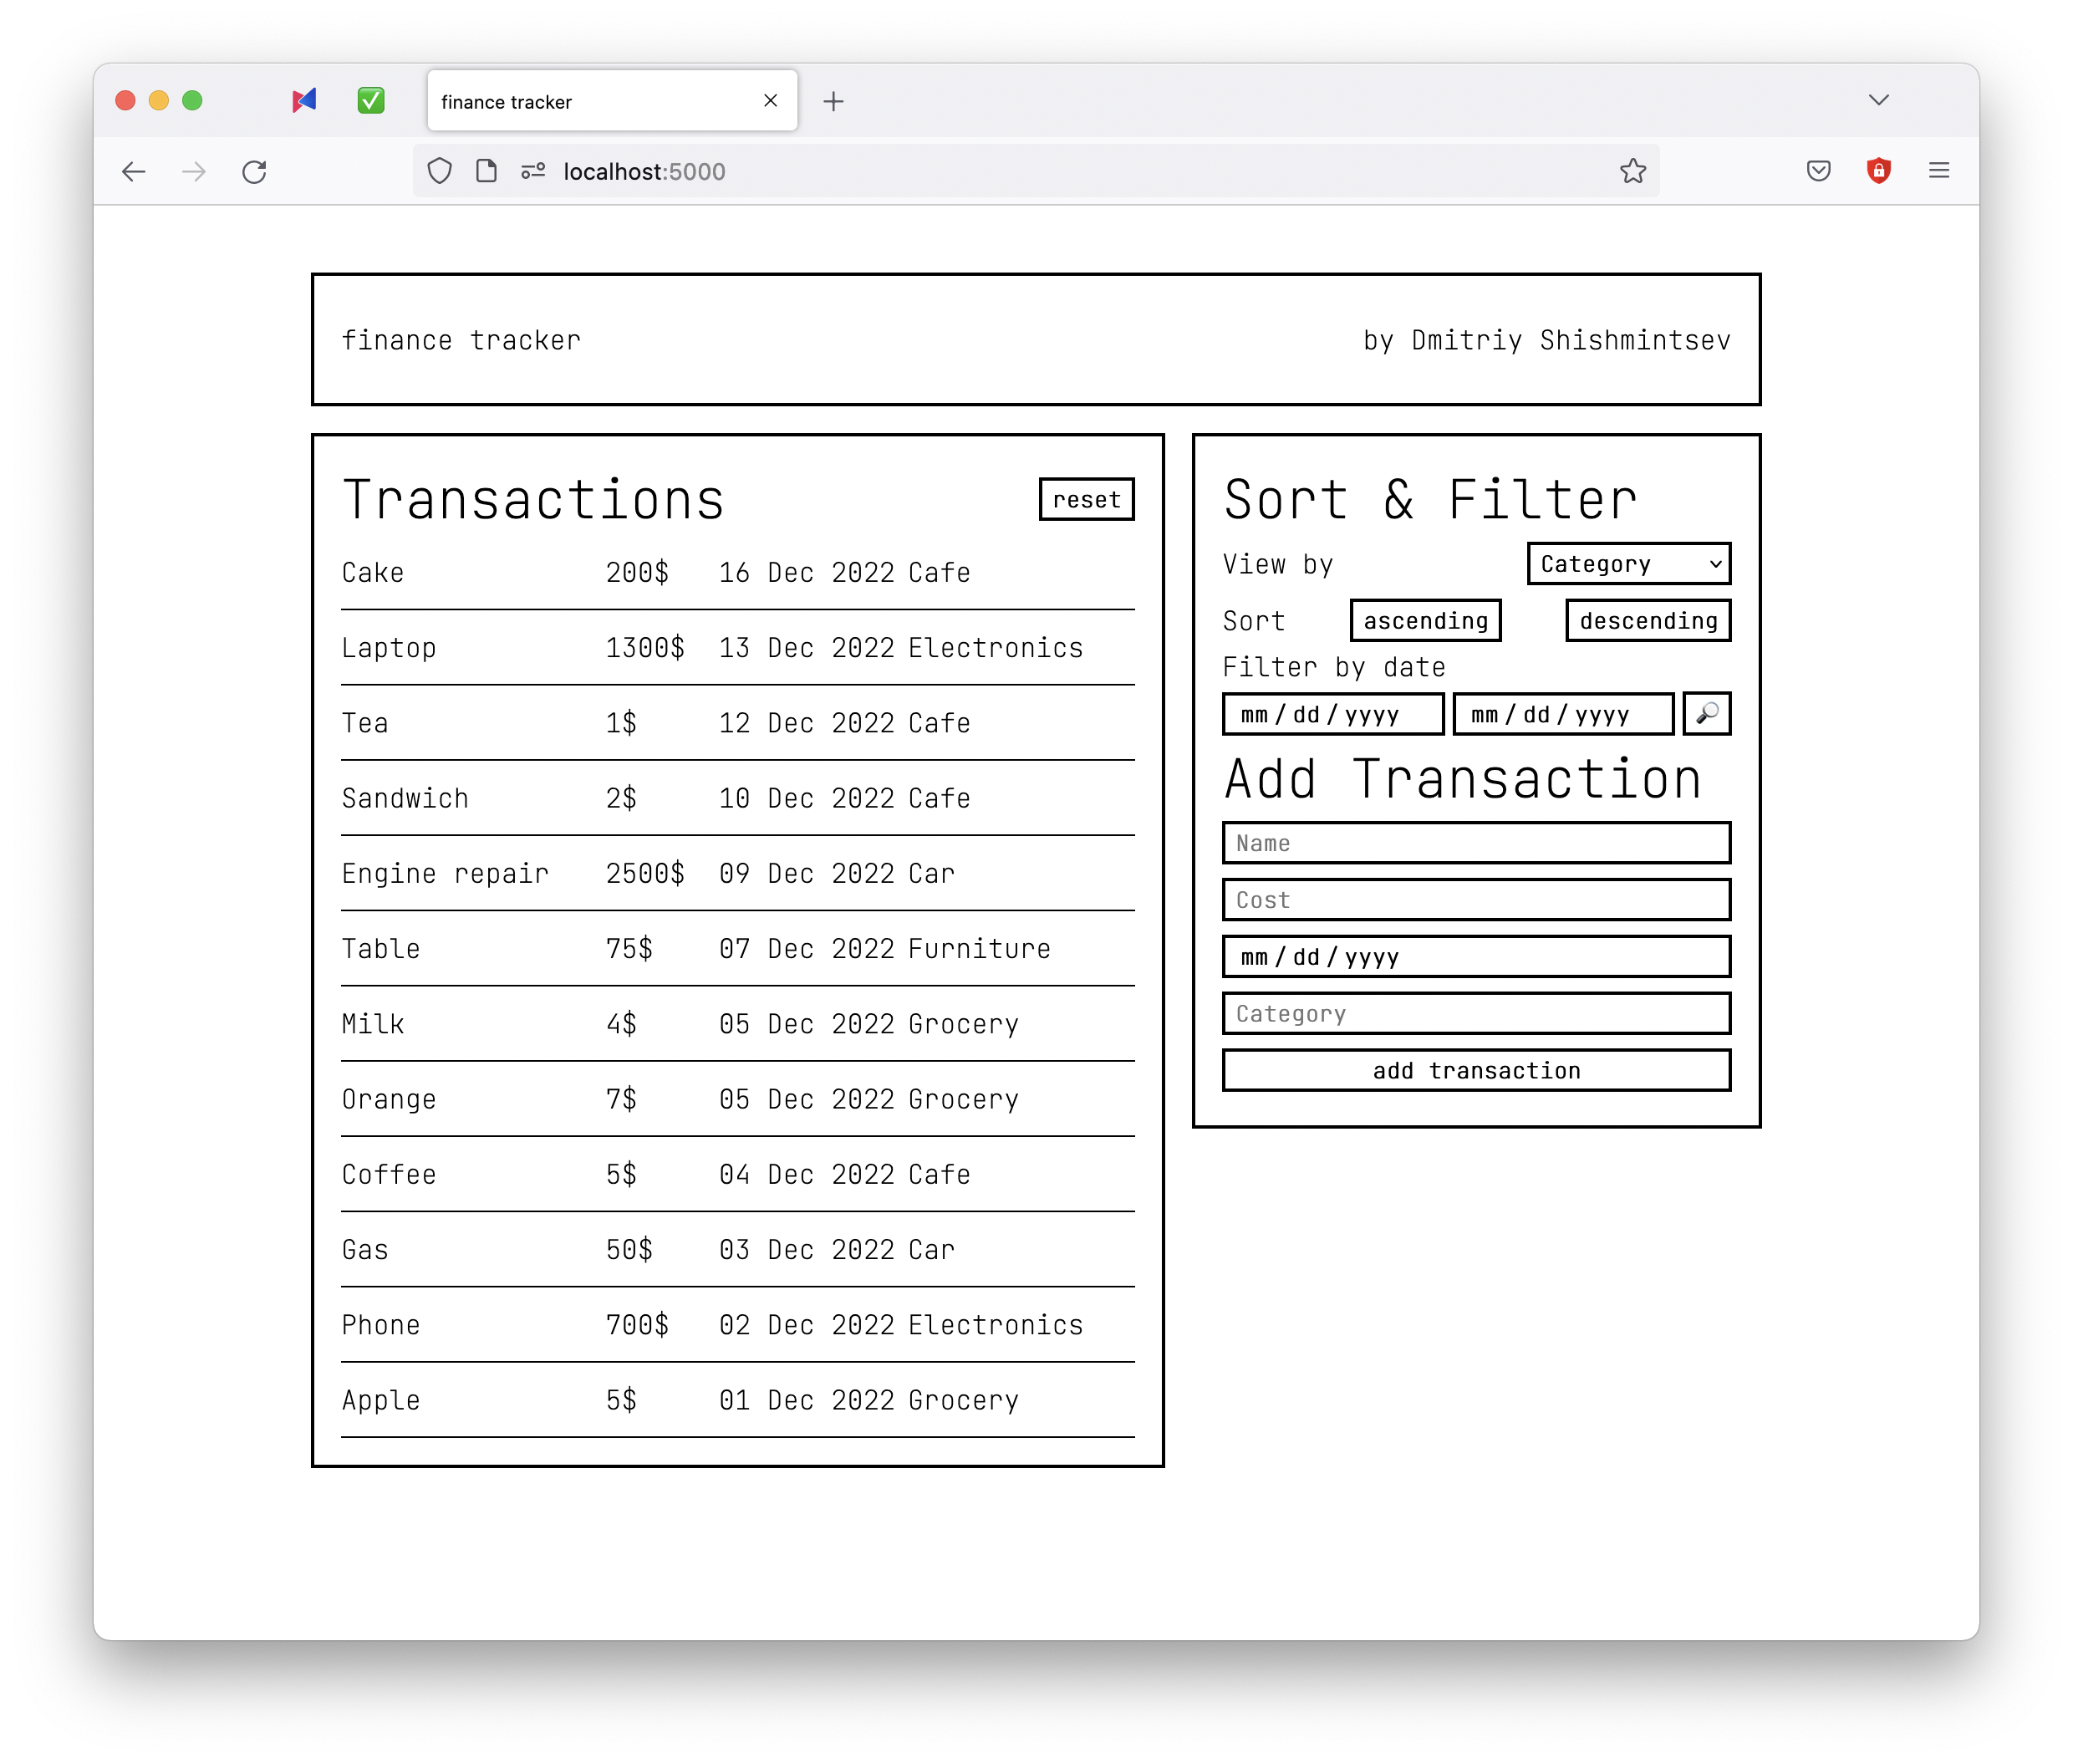
\includegraphics[width=1\linewidth]{int.png}
    \caption{ Интерфейс программы }
    \label{fig:d7}
\end{figure}

\conclusions

В результате данной работы была реализована программная модель инфокоммуникационной системы для контроля личных финансов. Была проанализирована предметная область. В процессе работы были использованы современные технологии и подходы к разработке программного обеспечения. 


\newpage
\begin{thebibliography}{99}
	\bibitem{bib1} 	\label{bib:bib1} SQLite3 - Официальный сайт (URL:\url{https://www.sqlite.org/})
    \bibitem{bib2} 	\label{bib:bib2} Python Docs - Официальный сайт (URL:\url{https://docs.python.org/3/})
    \bibitem{bib2} 	\label{bib:bib2} Flask  - Официальный сайт (URL:\url{https://flask.palletsprojects.com/en/2.2.x/})
\end{thebibliography}

\end{document}
